\documentclass{article}
\usepackage{amsmath, amssymb, amsthm, graphicx}
\usepackage[english]{babel}
\usepackage{hyperref}
\usepackage{tikz}
\usetikzlibrary{shapes.geometric}

\theoremstyle{plain}
\newtheorem{theorem}{Theorem}[section]
\newtheorem{lemma}[theorem]{Lemma}
\newtheorem{definition}[theorem]{Definition}
\newtheorem{example}[theorem]{Example}

\title{Guide to Convexity in Optimization}
\author{Mikhailova Olena}
\date{20.03.2025}

\begin{document}

\maketitle

\section{Introduction to Convexity}
Convexity is one of the most important concepts in optimization because it allows us to:
\begin{itemize}
    \item Guarantee that local minima are global minima
    \item Develop efficient optimization algorithms
    \item Analyze problems theoretically
\end{itemize}

\subsection{What Does "Convex" Mean?}
Imagine a simple bowl shape - this is convex. A saddle shape is non-convex. The key property is that if you draw a line between any two points on a convex object, the line stays entirely within the object.

\section{Convex Sets}
\subsection{Basic Definition}
\begin{definition}[Convex Set]
A set \( C \subseteq \mathbb{R}^n \) is \textbf{convex} if the line segment between any two points in \( C \) lies entirely in \( C \):
\[
\forall x,y \in C, \forall \theta \in [0,1]: \theta x + (1-\theta)y \in C
\]
\end{definition}

\subsection{Advanced Examples} % (new)
\begin{itemize}
    \item \textbf{Linear Matrix Inequality Solution Set}:
    \[
    \left\{x \in \mathbb{R}^k : \sum_{i=1}^k x_i A_i \preceq B\right\}
    \]
    where \( A_i, B \in \mathbb{S}^n \). Convexity follows because it's an affine pre-image of the PSD cone.
    
    \item \textbf{Conditional Probability Distributions}:
    The set of conditional distributions derived from convex joint distributions remains convex through linear-fractional transformations.
\end{itemize}

\subsection{Key Theorems}
\begin{theorem}[Separating Hyperplane]
For disjoint convex sets \( C,D \), there exists \( a,b \) such that:
\[
C \subseteq \{x : a^\top x \leq b\}, \quad D \subseteq \{x : a^\top x \geq b\}
\]
\end{theorem}

\begin{theorem}[Solution Set Convexity]
For convex optimization problems, the set of optimal solutions \( X_{\text{opt}} \) is convex.
\end{theorem}

\begin{proof}
Let \( x,y \in X_{\text{opt}} \). For \( t \in [0,1] \), define \( z = tx + (1-t)y \). By convexity:
\begin{align*}
g_i(z) &\leq t g_i(x) + (1-t)g_i(y) \leq 0 \\
A z &= t A x + (1-t)A y = b \\
f(z) &\leq t f(x) + (1-t)f(y) = f^*
\end{align*}
Thus \( z \in X_{\text{opt}} \).
\end{proof}


\subsection{Examples of Convex Sets}
\begin{itemize}
    \item \textbf{Norm balls}: All points within a certain distance from center
    \[ \{x : \|x\| \leq r\} \]
    
    \item \textbf{Hyperplanes and halfspaces}:
    \[ \{x : a^\top x = b\}, \quad \{x : a^\top x \leq b\} \]
    
    \item \textbf{Polyhedrons}: Solutions to systems of linear inequalities
    \[ \{x : Ax \leq b, Cx = d\} \]
    
    \item \textbf{Positive semidefinite cone} (for matrices):
    \[ \mathbb{S}_+^n = \{X \in \mathbb{R}^{n\times n} : X = X^\top, X \succeq 0\} \]
\end{itemize}

\subsection{Operations that Preserve Convexity}
\begin{itemize}
    \item \textbf{Intersection}: If \( C_1 \) and \( C_2 \) are convex, then \( C_1 \cap C_2 \) is convex
    
    \item \textbf{Affine transformations}: For convex \( C \), the set \( \{Ax + b : x \in C\} \) is convex
    
    \item \textbf{Linear-fractional transformations}: For convex \( C \), the set \( \left\{\frac{Ax+b}{c^\top x + d} : x \in C\right\} \) is convex
\end{itemize}

\section{Convex Functions}
\subsection{Basic Definition}
\begin{definition}[Convex Function]
A function \( f : \mathbb{R}^n \to \mathbb{R} \) is \textbf{convex} if its domain is convex and:
\[
f(\theta x + (1-\theta)y) \leq \theta f(x) + (1-\theta)f(y) \quad \forall x,y \in \text{dom}(f), \theta \in [0,1]
\]
\end{definition}

\begin{center}
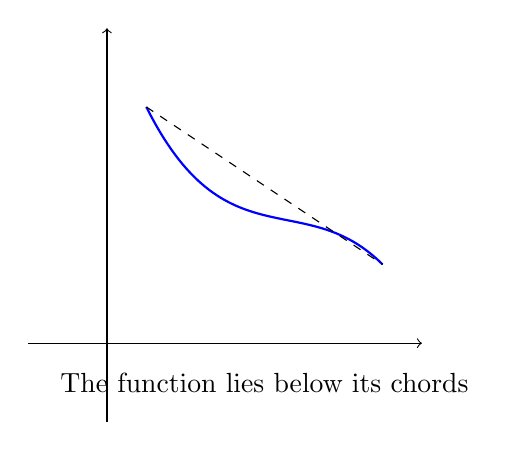
\begin{tikzpicture}
\draw[->] (-1,0) -- (4,0);
\draw[->] (0,-1) -- (0,4);
\draw[blue, thick] (0.5,3) .. controls (1.5,1) and (2.5,2) .. (3.5,1);
\draw[dashed] (0.5,3) -- (3.5,1);
\node at (2,-0.5) {The function lies below its chords};
\end{tikzpicture}
\end{center}

\subsection{Extended Properties} % (new)
\begin{itemize}
    \begin{theorem}[Partial Minimization]
If \( g(x,y) \) is convex and \( C \) is convex, then \( f(x) = \min_{y \in C} g(x,y) \) is convex.
\end{theorem}
    
    \item \textbf{Composition Rules}:
    \begin{itemize}
        \item Convex + non-decreasing \(\circ\) convex = convex
        \item Convex + non-increasing \(\circ\) concave = convex
        \item Affine composition preserves convexity: \( f(Ax+b) \)
    \end{itemize}
\end{itemize}

\subsection{Important Properties}
\begin{itemize}
    \begin{theorem}[Epigraph Characterization]
\( f \) is convex \(\iff\) its epigraph \( \text{epi}(f) = \{(x,t) : f(x) \leq t\} \) is convex.
\end{theorem}
    
    \begin{theorem}[First-Order Characterization]
For differentiable \( f \):
\[
f \text{ convex} \iff f(y) \geq f(x) + \nabla f(x)^\top (y - x) \quad \forall x,y
\]
\end{theorem}

\begin{theorem}[Second-Order Characterization]
For twice differentiable \( f \):
\[
f \text{ convex} \iff \nabla^2 f(x) \succeq 0 \quad \forall x
\]
\end{theorem}
\end{itemize}

\subsection{Important Function Classes} % (new)
\begin{itemize}
    \item \textbf{Indicator Function}:
    \[
    I_C(x) = \begin{cases} 
    0 & x \in C \\
    \infty & \text{otherwise}
    \end{cases}
    \]
    Convex when \( C \) is convex
    
    \item \textbf{Support Function}:
    \[
    I_C^*(x) = \sup_{y \in C} x^\top y
    \]
    Always convex (even for non-convex \( C \))
\end{itemize}

\subsection{Examples of Convex Functions}
\begin{itemize}
    \item \textbf{Affine functions}: \( f(x) = a^\top x + b \)
    
    \item \textbf{Quadratic functions}: \( f(x) = \frac{1}{2}x^\top Q x + b^\top x + c \) (when \( Q \succeq 0 \))
    
    \item \textbf{Norms}: \( \|x\|_p \) for \( p \geq 1 \)
    
    \item \textbf{Exponential}: \( e^{ax} \)
    
    \item \textbf{Log-sum-exp}: \( \log(\sum e^{x_i}) \)
\end{itemize}

\subsection{Strong Convexity}
\begin{definition}[Strongly Convex Function]
A function \( f \) is \textbf{\(\mu\)-strongly convex} if:
\[
f(y) \geq f(x) + \nabla f(x)^\top (y - x) + \frac{\mu}{2}\|y - x\|^2
\]
This means the function grows at least as fast as a quadratic function.
\end{definition}

\begin{theorem}[Hessian Characterization]
For twice differentiable \( f \):
\[
f \text{ \(\mu\)-strongly convex} \iff \nabla^2 f(x) \succeq \mu I \quad \forall x
\]
\end{theorem}

\subsection{Algorithmic Implications}
\begin{itemize}
    \item Enables linear convergence rates
    \item Provides error bounds:
    \[
    \frac{1}{2\mu}\|\nabla f(x)\|^2 \geq f(x) - f^*
    \]
    \item Guarantees unique global minimum
    \item Leads to faster convergence in optimization algorithms
    \item For twice differentiable \( f \), equivalent to \( \nabla^2 f(x) \succeq \mu I \)
\end{itemize}

\section{Convex Optimization Problems}
\subsection{Standard Form}
A convex optimization problem has the form:
\[
\begin{aligned}
\min_{x} \quad & f(x) \\
\text{s.t.} \quad & g_i(x) \leq 0, \quad i = 1,...,m \\
& a_j^\top x = b_j, \quad j = 1,...,p
\end{aligned}
\]
where:
\begin{itemize}
    \item \( f \) and \( g_i \) are convex functions
    \item Equality constraints are affine
\end{itemize}

\subsection{Problem Transformations} % (new)
\begin{itemize}
    \item \textbf{Eliminating Equality Constraints}:
    Express \( x = My + x_0 \) where \( M \) spans nullspace of \( A \)
    
    \item \textbf{Introducing Slack Variables}:
    Convert \( g_i(x) \leq 0 \) to \( g_i(x) + s_i = 0 \) with \( s_i \geq 0 \)
    
    \item \textbf{Geometric Programming}:
    Non-convex posynomials become convex after log-transform:
    \[
    \min_y \log\sum e^{a_k^\top y + b_k} \quad \text{s.t.} \quad \log\sum e^{c_i^\top y + d_i} \leq 0
    \]
\end{itemize}

\subsection{Key Properties}
\begin{itemize}
    \begin{theorem}[Global Optimality]
For convex problems, any local minimum is global.
\end{theorem}

\begin{theorem}[Solution Uniqueness]
If \( f \) is strictly convex, the solution is unique.
\end{theorem}
    
\begin{theorem}[Optimality condition]: For differentiable \( f \), \( x^* \) is optimal iff
    \[ \nabla f(x^*)^\top (y - x^*) \geq 0 \quad \forall y \text{ feasible} \]
    \end{theorem}
\end{itemize}

\subsection{Solution Characteristics} % (new)
\begin{itemize}
    \item \textbf{Feasibility}: A point \( x \) is feasible if \( x \in \bigcap\text{dom}(g_i) \), \( g_i(x) \leq 0 \), and \( Ax = b \)
    
    \item \textbf{Active Constraints}: Inequality \( g_i \) is active at \( x \) if \( g_i(x) = 0 \)
    
    \item \epsilon\textbf{-Suboptimality}: \( x \) is \( \epsilon \)-suboptimal if \( f(x) \leq f^* + \epsilon \)
\end{itemize}

\subsection{Important Examples}
\begin{itemize}
    \item \textbf{Linear Programs (LP)}:
    \[ \min_x c^\top x \quad \text{s.t.} \quad Ax \leq b \]
    
    \item \textbf{Quadratic Programs (QP)}:
    \[ \min_x \frac{1}{2}x^\top Q x + c^\top x \quad \text{s.t.} \quad Ax \leq b \]
    
    \item \textbf{Semidefinite Programs (SDP)}:
    \[ \min_X \langle C, X \rangle \quad \text{s.t.} \quad \mathcal{A}(X) = b, X \succeq 0 \]
\end{itemize}

\section{Applications}
\subsection{Lasso Regression}
\[
\min_\beta \|y - X\beta\|_2^2 + \lambda\|\beta\|_1
\]
\begin{itemize}
    \item Convex despite non-differentiable \( \ell_1 \)-norm
    \item Promotes sparse solutions
\end{itemize}

\subsection{Robust Lasso Variant} % (new)
With Huber loss for outlier resistance:
\[
\min_\beta \sum_{i=1}^n \rho(y_i - x_i^\top\beta) + \lambda\|\beta\|_1
\]
where \( \rho(z) = \begin{cases} 
\frac{1}{2}z^2 & |z| \leq \delta \\
\delta|z| - \frac{1}{2}\delta^2 & \text{otherwise}
\end{cases} \). Remains convex as Huber loss is convex.

\subsection{Support Vector Machines}
\[
\min_{w,b} \frac{1}{2}\|w\|_2^2 + C\sum_{i=1}^n \max(0, 1 - y_i(w^\top x_i + b))
\]
\begin{itemize}
    \item Convex objective with piecewise linear constraints
    \item Can be rewritten as a quadratic program
\end{itemize}

\subsection{SVM Duality} % (new)
The dual SVM formulation reveals convex structure:
\[
\max_\alpha \sum_{i=1}^n \alpha_i - \frac{1}{2}\sum_{i,j} \alpha_i\alpha_j y_iy_j x_i^\top x_j \quad \text{s.t.} \quad 0 \leq \alpha_i \leq C
\]
Demonstrates convex quadratic programming structure.

\section{Why Convexity Matters}
\begin{itemize}
    \item \textbf{Reliable optimization}: No need to worry about getting stuck in local minima
    
    \item \textbf{Efficient algorithms}: Specialized methods (gradient descent, interior point) work well
    
    \item \textbf{Theoretical guarantees}: Can prove convergence rates and complexity bounds
    
    \item \textbf{Recognizable structure}: Many problems can be reformulated as convex programs
\end{itemize}

\section{Algorithmic Implications} % (new)
\subsection{Why Convexity Helps Optimization}
\begin{itemize}
    \item \textbf{No Spurious Local Minima}: Gradient descent won't get stuck in poor solutions
    
    \item \textbf{Predictable Convergence}:
    \begin{itemize}
        \item \( O(1/\epsilon) \) iterations for convex + smooth
        \item Linear convergence (\( O(\log 1/\epsilon) \)) for strongly convex
    \end{itemize}
    
    \item \textbf{Simple Stopping Criteria}: \( \|\nabla f(x)\| < \epsilon \) guarantees near-optimality
\end{itemize}

\subsection{Hierarchy of Convex Programs} % (new)
\begin{center}
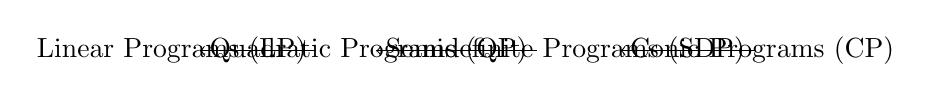
\begin{tikzpicture}
\node (LP) at (0,0) {Linear Programs (LP)};
\node (QP) at (2.5,0) {Quadratic Programs (QP)};
\node (SDP) at (5,0) {Semidefinite Programs (SDP)};
\node (CP) at (7.5,0) {Conic Programs (CP)};
\draw[->] (LP) edge (QP) (QP) edge (SDP) (SDP) edge (CP);
\end{tikzpicture}
\end{center}
Each class extends the previous one while maintaining convexity properties.

\section{Recognizing Convexity}
To verify if a problem is convex:
\begin{enumerate}
    \item Check if the objective is convex (use definitions or derivative tests)
    \item Verify all inequality constraints are convex
    \item Ensure equality constraints are affine
    \item Confirm the domain is convex
\end{enumerate}

\begin{itemize}
    \item \textbf{Significant Counterexample}: Geometric programs appear non-convex but become convex under logarithmic transformation
\end{itemize}

\section{Common Mistakes}
\begin{itemize}
    \item Assuming all quadratics are convex (must check \( Q \succeq 0 \))
    \item Forgetting to verify convexity of constraints
    \item Treating equality constraints as inequalities
    \item Overlooking domain issues (e.g., log(x) requires x > 0)
\end{itemize}

\section{Conclusion}
Convexity provides a powerful framework for optimization problems:
\begin{itemize}
    \item Clear geometric interpretation
    \item Strong theoretical guarantees
    \item Wide range of applications
    \item Systematic approach to problem formulation
\end{itemize}

\end{document}